%This is a LaTeX template for homework assignments
\documentclass{article}
\usepackage[utf8]{inputenc}
\usepackage{amsmath,enumerate}
\usepackage[]{mcode}
\usepackage{graphicx}
\usepackage{float}


\begin{document}

\section*{Assignment 0}
Name: Julien Neves
\\Student Number: 260462227
\\Date: January 30, 2017

\subsection*{Problem 1}

\subsubsection*{4.1 - Derivative-Free Methods}


\subsubsection*{4.2 - Newton-Rhapson Method}


\subsubsection*{4.3 - Quasi-Newton Methods}


The Quasi-Newton methods employ the same strategy as the Newton method, but restrict the Hessian matrix to be Negative-definite approximation. This insures that the value function will increase at every step.

Like the Newton method, we get the that the direction we should take to optimize our function is given by
$$
d^{(k)}= - B^{(k)}f'(x^{(k)})
$$
where $B^{(k)}$ is the approximation to the Hessian $f'(x^{(k)})$ is the gradient evaluated at $x^{(k)}$.

Then, the updating of $x^{(k)}$ is given by the following formula.
$$
x^{(k+1)}= x^{(k)}-s^{(k)}d^{(k)}
$$
where $s^{(k)}$ is scaling factor for the $d^{(k)}$. If $B^{(k)}$ is the actual Hessian matrix and $s^{(k)}$ is set equal to one, it is easy to see that we are back at the original Netwon method.

Now, the choice of $B^{(k)}$ is important in terms of efficiency. The easiest choice for $B^{(k)}$ is to set it equal to the negative identity matrix $-I$. This insures the that $B^{(k)}$ is negative definite, but at the same time this is not the most optimal way to go about it. This choice of $B^{(k)}$ let's $d^{(k)}= f'(x^{(k)})$ which is the equivalent to having a Newton-step in the direction of the gradient. This method is now as the method of steepest ascent. 

Note that to satisfy the Quasi-Newton method, the matrix $B^{(k)}f'(x^{(k)})$ is require to satisfy two conditions:

\begin{enumerate}
\item Quasi-Newton Condition: 
$$
d^{(k)}= B^{(k+1)}[f'(x^{(k)}+d^{(k)})-f'(x^{(k)})]
$$
\item The inverse $B^{(k)}$ needs to be both symmetric and negative definite
\end{enumerate}

Two methods that satisfy this are the Davidon-Fletcher-Powell (DFP) and Broyden-Fletcher-Goldfard-Shano (BFGS) algorithms.

For the DFP algorithm, $B^{(k)}$ is updated in the following way:
$$
B^{(k+1)} = B^{(k)} + \frac{dd'}{d'u}-\frac{B^{(k)}dd'B^{(k)}}{u'B^{(k)}u}
$$
where $d=x^{(k+1)}-x^{(k)}$ and $u=f'(x^{(k+1)})-f'(x^{(k)})$ 

For the BFGS algorithm, $B^{(k)}$ is updated in the following way:
$$
B^{(k+1)} = B^{(k)} + \frac{1}{d'u}\left(wd'+dw'-\frac{w'u}{d'u}dd'\right)
$$
where $d=x^{(k+1)}-x^{(k)}$, $u=f'(x^{(k+1)})-f'(x^{(k)})$ and $w=d-B^{(k)}u$

BFGS is known to be superior to the DFP algorithm which both perfom better than the steepest ascent method usually.

One issue that the Quasi-Newton methods have is that due to the possible explosive nature of $\frac{1}{d'u}$. One way to prevent for this is to test that the following
$$
|d'u|< \epsilon ||d|| ||u||
$$
if it doesn't hold, we can either stop updating $B{(k)}$ or reset it to a negative identity matrix.
\subsubsection*{4.4 - Line Search Methods}

Like previously stated we might want to change our $s$ in our Quasi-Newton methods to improve our search. For example the golden search method is an example of linear search method.

Other example of linear search methods are for example the Armijo search and the Goldstein search.

For the Arminjo search, our goal is to find the minimum power of $j$ such that
$$
\frac{f(x+sd)-f(x)}{s}\geq \mu f'(x)^Td
$$
where $s=\rho^j$, $0<\rho <1$, and $0<\mu<0.5$. The basic goal is of this method is to start from a step-size of one, an backtrack until the slope on the lefthand side is a fraction $\mu$ of the slope on the righthand side.

For the Goldstein search, we find any values of $s$ such that
$$
\mu_0 f'(x)^Td \leq \frac{f(x+sd)-f(x)}{s}\leq \mu_1 f'(x)^Td
$$
for some values of $0<\mu_0\leq 0.5 \leq \mu_1 <0$. Note that in the case of Goldstein method, we only have a stopping rule and not a method of selecting candidates. 

One way to select a candidate $s$ in this case, is to double $s$ until we find a point that is such that it respect the Goldstein criterion or that is such that $
\mu_0 f'(x)^Td > \frac{f(x+sd)-f(x)}{s}
$ which we can then backtrack to a point that respect the criterion. 

Another method is to start with $s=1$ and $s$ is updated using the cubic approximation of the objective function until an appropriate point it found. Generaly this method will be fast, and better than other line search methods in most cases (especially if the function is smooth).

Finally the golden search, use the same procedure as described in $4.1$ to find an step size by setting a bracket of possible values of $s$ and reducing it until we are satisfied. 

\subsection*{Problem 2}

\subsubsection*{3.3}

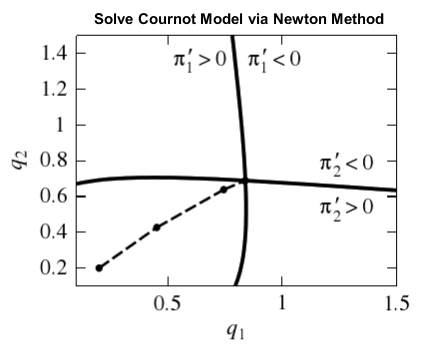
\includegraphics[scale=0.7]{3_3}

On this figure, we see an example of the Cournot problem where $\eta=1.6$, $c_1=0.6$, and $c_2=0.8$. As we can see, the best response is that at the intersection of the reactions curves of both players. Using the Newton method and starting at $q_1=q_2=0.2$, it takes roughly three steps to reach the equilibrium. 

\subsubsection*{4.1}

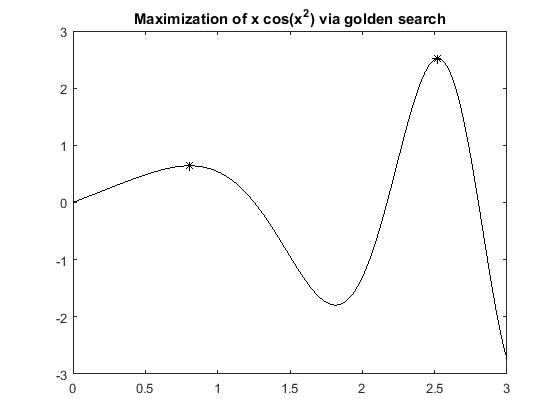
\includegraphics[scale=0.7]{4_1}

Using golden search, we maximizes the function $x\cos (x^2)$. With this algorithm, we reach $x=0.8083$. It is straightforward to see that it is only a local maximum and not a global one. In fact, at $x=2.5$ we have a global maximum on $x=[0,3]$. This is problem arises from the fact that the optimand is not concave

\subsubsection*{4.3}

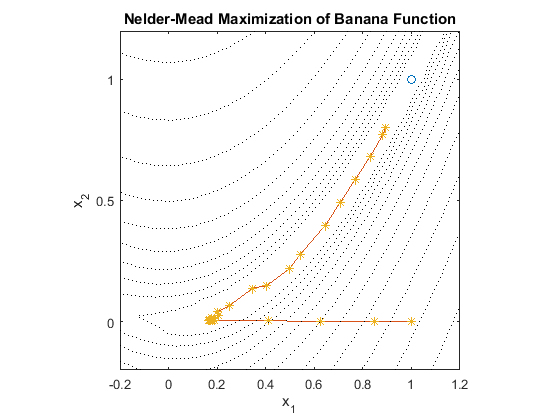
\includegraphics[scale=0.7]{4_3}

On this figure, we maximizes the banana function $f(x)=-100(x_2-x_1^2)^2-(1-x_1)^2$ using the Nelder-Mead algorithm. It reaches its stopping point at $x=(1,1)$ which is the global maximum. It takes the Nelder-Mead method 55 steps to reach this global maximum. The Nelder-Mead algorithm is based on evaluating the vertices of a simplex and then updating the simplex through reflection, expansion, contraction and shrinkage depending on the value of the vertices in order to converge to the maximum.
\clearpage

\appendix
\section*{Appendix - Code}

\lstinputlisting{demslv12.m}
\clearpage

\lstinputlisting{demopt01.m}
\clearpage

\lstinputlisting{demopt03.m}
\clearpage
\end{document}